Wie in Abbildung \ref{fig: controller architektur} zu sehen ist, umfasst der Controller die Schichten Physical Layer (PHY) und Link Layer (LL). Über dem Controller ist der Logical Link Control And Adaption Protocol (L2CAP) Layer in grau dargestellt, da er nicht Teil des Controllers sondern des Hosts ist.

\begin{figure}[H]
    \centering
    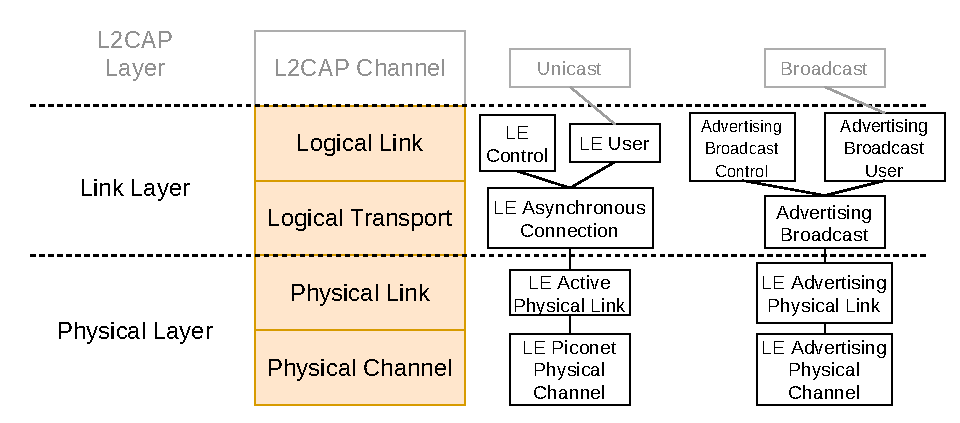
\includegraphics[width=1\textwidth]{graphics/controller_layers.pdf}
    \caption[Architektur des Physical Layers und des Link Layers]{Architektur des Physical Layers und des Link Layers; in Anlehnung an \cite{BtSpec4.0_fig_145} und \cite{BtSpec4.0_fig_151}}
    \label{fig: controller architektur}
\end{figure}

Der Physical Layer unterteilt sich weiter in die Physical Channels und die Physical Links, während der Link Layer sich in Logical Transports und Logical Links aufteilt. In den Schichten bzw. ihren Untergliederungen wird definiert, wie Anwendungsdaten und Kontrollsignale innerhalb Verbindungen bzw. Advertisements übertragen werden. Bezüglich des L2CAP Layers werden Anwendungsdaten entweder in Form eines Unicasts oder Broadcasts übertragen.